% !TeX spellcheck = it_IT
\newpage
\section{Software services}
\subsection{REST}
REST (REpresentational State Trasfer) è uno stile architetturale sviluppato come modello astratto per il Web.\\
Ogni azione causa il passaggio dell'applicazione allo stato successivo tramite il trasferimento dello stato corrente.\\
Si basa sui seguenti principi:
\begin{itemize}
	\item \textbf{URIs (Uniform Resource Identifier)}: identificazione delle risorse in maniera \textit{univoca} e \textit{universale}, ad esempio gli indirizzi Web
	\item \textbf{Interfaccia uniforme}: ad esempio per il protocollo HTTP, l'utente invoca dei metodi predefiniti:
	\begin{itemize}
		\item \textit{POST} e \textit{PUT} per creare e aggiornare risorse
		\item \textit{DELETE} per eliminare una risorsa
		\item \textit{GET} per ottenere lo stato corrente di una risorsa
	\end{itemize}
	\item \textbf{Messaggi autoesplicativi}: ogni richiesta contiene abbastanza \textit{contesto} per riuscire a comprendere il messaggio. Inoltre le risorse sono \textit{separate} dalla loro rappresentazione in modo da poter essere accedute in diversi formati
	\item \textbf{Interazioni stateful tramite hyperlinks}: data la natura stateless, per fornire interazioni stateful si utilizzano trasferimenti espliciti di stato tramite hyperlinks
\end{itemize}
\subsubsection{Negoziazione}
Quando viene richiesta una risorsa, vanno specificati i formati accettabili. Il server poi risponde con la risorsa nel formato più appropriato o eventualmente con il codice di errore 406.
\begin{center}
	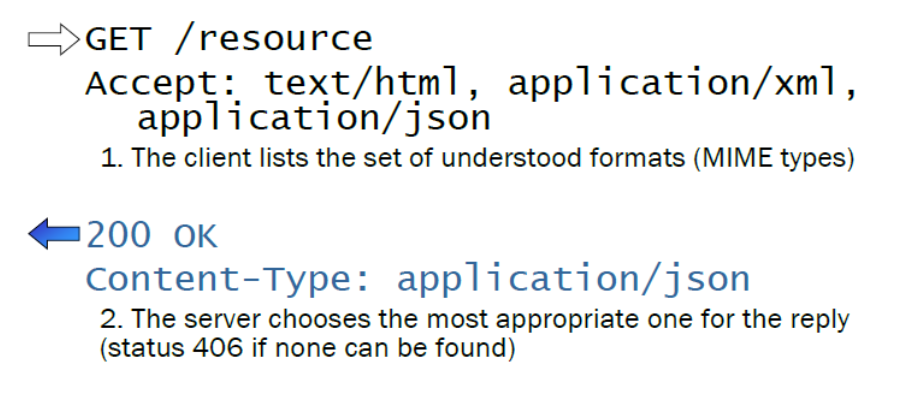
\includegraphics[scale=0.2]{negotiation.png}
\end{center}
\subsubsection{Design}
Il design deve seguire i seguenti passaggi:
\begin{enumerate}
	\item Identificare le risorse che devono essere esposte come servizi
	\item Modellare le relazioni tra le risorse tramite gli \textit{hyperlinks}
	\item Definire gli URIs seguendo le seguenti guidelines:
	\begin{itemize}
		\item Meglio i sostantivi dei verbi
		\item Brevità
		\item Utilizzare i template per costruire ed elaborare URIs parametrici
		\item Non cambiarli, nel caso utilizzare il reindirizzamento
	\end{itemize}
	\item Definire quali metodi sono applicabili alla risorsa
	\item Progettare e documentare la rappresentazione delle risorse
	\item Implementare e rilasciare il servizio
	\item Testing
\end{enumerate}
\subsubsection{Riepilogo}
L'architettura REST è \textbf{semplice} (utilizza standard famosi e infrastruttura già presente), \textbf{leggera} (sia per i protocolli utilizzati che per i messaggi) e \textbf{scalabile}. Di contro però i client possono richiedere troppi o troppi pochi dati, possono fare un numero limitato di richieste e le convenzioni per la nomenclatura sono inconsistenti.